\documentclass[11pt]{article}
\usepackage[T1]{fontenc}
\usepackage{lmodern}
\usepackage[margin=1in]{geometry}
\usepackage{amsmath,amssymb,amsthm,mathtools}
\usepackage{graphicx}
\usepackage{tikz}
\usepackage[hidelinks]{hyperref}
\newtheorem{theorem}{Theorem}
\newtheorem{corollary}[theorem]{Corollary}
\newtheorem{lemma}[theorem]{Lemma}
\newtheorem{remark}[theorem]{Remark}
\DeclareMathOperator{\supp}{supp}
\setlength{\emergencystretch}{3em}
\title{The $\alpha=1$ Maz'ya endpoint:\\collapse to ordinary function-space inclusion}
\author{Run \texttt{fa\_banach\_001}, lane 18 (\texttt{agent\_lane\_18})}
\date{12 August 2026}

\begin{document}
\maketitle

\begin{abstract}
The source leaves the case $\alpha=1$ in Maz'ya classes as one branch of a
larger open program.  We prove a sharp endpoint theorem for the inhomogeneous
Sobolev-domain problem.  A single bounded coiled exponential horn in
$\mathcal J_1$ supports
translated smooth bumps whose measures form a geometric scale.  Consequently,
for any Orlicz domain $L^A$, any rearrangement-invariant target $Y$, and every
order $m\geq1$, an embedding $W^mL^A(\Omega)\hookrightarrow Y(\Omega)$ valid
for all $\Omega\in\mathcal J_1$ is equivalent to the ordinary inclusion
$L^A(0,1)\hookrightarrow Y(0,1)$.  Applied to the formal endpoint family
$L^{\infty,q;-1-1/q}$, this gives nonexistence of a largest Orlicz domain for
$q<\infty$, but the largest domain $\exp L$ when $q=\infty$.
\end{abstract}

\section{Source question and precise scope}

Ber\'anek's paper treats measure-one Euclidean domains whose isoperimetric
profiles satisfy $I_\Omega(t)\gtrsim t^\alpha$.  Its reduction and optimality
theorems assume $\alpha<1$.  The final remark explicitly leaves several much
broader directions open:

\begin{center}

\includegraphics[width=.93\textwidth]{figures/open_problem_crop.png}
\end{center}

The statement does not pose one theorem encompassing all four directions.
This packet selects the precise first branch: universal, inhomogeneous
Sobolev embeddings over the endpoint class $\mathcal J_1$.  The result below
also classifies the formal $\alpha=1$ endpoint of the Lorentz--Zygmund target
scale used in the source.

\section{Definitions}

All domains are bounded and have Lebesgue measure one.  If $E\subset\Omega$ has finite
perimeter, write $P(E,\Omega)$ for its relative perimeter.  For
$0<t\leq\tfrac12$, set
\[
 I_\Omega(t)=\inf\{P(E,\Omega):E\subset\Omega,
                       \ t\leq |E|\leq\tfrac12\}.
\]
The endpoint Maz'ya class is
\[
 \mathcal J_1=\{\Omega:I_\Omega(t)\geq c_\Omega t
                 \text{ for }0<t\leq\tfrac12\}.
\]

Let $Y$ be a rearrangement-invariant (r.i.) Banach function space, with
representation space $Y(0,1)$.  If $A$ is a Young function, $L^A$ denotes the
corresponding Orlicz space with Luxemburg norm.  We use the inhomogeneous norm
\[
 \|u\|_{W^mL^A(\Omega)}=\sum_{j=0}^m
                    \|\,|\nabla^j u|\,\|_{L^A(\Omega)}.
\]
The zeroth-order term is essential at this endpoint.

For $1\leq q<\infty$, define
\[
 Y_q=L^{\infty,q;-1-1/q}(0,1),\qquad
 \|f\|_{Y_q}^q=
 \int_0^1\frac{f^*(t)^q}{t\,[\log(2/t)]^{q+1}}\,dt,
\]
with the usual equivalent r.i. norm.  For $q=\infty$,
\[
 \|f\|_{Y_\infty}=\sup_{0<t<1}
       \frac{f^*(t)}{\log(2/t)},
 \qquad Y_\infty=\exp L.
\]

\section{Result and proof intuition}

\begin{theorem}[endpoint collapse]\label{thm:collapse}
Let $n\geq2$, $m\geq1$, let $Y$ be an r.i. Banach function space on a
probability space, and let $A$ be a Young function.  The following are
equivalent.
\begin{enumerate}
\item For every $\Omega\in\mathcal J_1$,
\[
 W^mL^A(\Omega)\hookrightarrow Y(\Omega),
\]
where the embedding constant may depend on $\Omega$.
\item $L^A(0,1)\hookrightarrow Y(0,1)$.
\end{enumerate}
In fact, one fixed domain $\Omega_*$ suffices to deduce (2) from (1).
\end{theorem}

The mechanism is geometric.  The domain $\Omega_*$ is a bounded tube around an
infinite spiral, with exponentially shrinking cross-section.  Moving a fixed
smooth bump one unit farther along the tube multiplies the measure of its
support by a fixed factor, without changing the size of any derivative.  The
coiling keeps the domain bounded while preserving uniform longitudinal
geometry.  Disjoint translated bumps therefore reproduce every geometrically
discretized measurable function.  A universal Sobolev embedding on
$\mathcal J_1$ must already bound all such functions before differentiation is
used.

\begin{center}
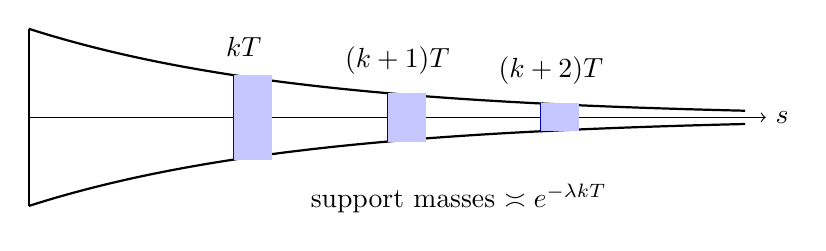
\begin{tikzpicture}[x=1.3cm,y=.9cm]
  \draw[->] (0,0) -- (7.2,0) node[right] {$s$};
  \draw[thick,domain=0:7,samples=80] plot (\x,{1.25*exp(-\x/2.7)});
  \draw[thick,domain=0:7,samples=80] plot (\x,{-1.25*exp(-\x/2.7)});
  \draw[thick] (0,-1.25)--(0,1.25);
  \foreach \x/\lab in {2.0/$kT$,3.5/$(k+1)T$,5.0/$(k+2)T$}{
    \fill[blue!22] (\x,-{1.25*exp(-\x/2.7)}) rectangle
       ({\x+.38},{1.25*exp(-\x/2.7)});
    \draw[blue!70!black] (\x,-{1.25*exp(-\x/2.7)})--
       (\x,{1.25*exp(-\x/2.7)});
    \node[above] at ({\x+.1},{1.25*exp(-\x/2.7)+.13}) {\lab};
  }
  \node at (4.2,-1.15) {support masses $\asymp e^{-\lambda kT}$};
\end{tikzpicture}
\end{center}

\section{The bounded coiled exponential horn}

We first build a bounded curve of infinite length with uniform local geometry.
For large $t$, consider the planar spiral
\[
 \widetilde\gamma(t)=
 \big((1+(t+2)^{-1})\cos t,
      (1+(t+2)^{-1})\sin t,0,\ldots,0\big).
\]
Reparametrize a tail of this curve by arclength, writing it as
$\gamma:[0,\infty)\to\mathbb R^n$.  The curve stays in a bounded annulus, has
infinite length, and all its arclength derivatives are bounded.  Successive
turns at parameter size $s$ are separated by a distance comparable to
$s^{-2}$.  Choose a smooth orthonormal normal frame
$N_1(s),\ldots,N_{n-1}(s)$ with bounded derivatives and put
\[
 \varepsilon(s)=\varepsilon_0e^{-\beta s},\qquad
 F(y,s)=\gamma(s)+\varepsilon(s)
       \sum_{i=1}^{n-1}y_iN_i(s),\qquad y\in B, s>0,
\]
where $B$ is the unit ball in $\mathbb R^{n-1}$.  For sufficiently small
$\varepsilon_0>0$, exponential decay is faster than the polynomial separation
of the turns, so $F$ is injective.  Its image $\Omega_0$ is a bounded open
connected tube.  After one fixed homothety, call the resulting measure-one
domain $\Omega_*$.  This homothety affects only fixed constants below.

\begin{lemma}\label{lem:horn}
$\Omega_*$ is bounded, $|\Omega_*|=1$, and
$I_{\Omega_*}(t)\asymp t$ for $0<t\leq\tfrac12$.  In particular,
$\Omega_*\in\mathcal J_1$.
\end{lemma}

\begin{proof}
Let $\lambda=\beta(n-1)$.  The standard tube-Jacobian formula and bounded
curvature give, uniformly in $(y,s)$,
\[
 J_F(y,s)=\varepsilon(s)^{n-1}(1+O(\varepsilon(s)))
          \asymp e^{-\lambda s}.
\]
Thus $0<|\Omega_0|<\infty$, and the announced homothety normalizes its volume.

The uniform probability measure on the bounded ball $B$ satisfies an
$L^1$ Poincar\'e inequality, as does the one-sided exponential probability
measure $e^{-\lambda s}ds$.  The elementary Fubini argument for the mean in
the two variables tensorizes these inequalities.  Since $J_F$ is comparable
to the product density and the differential of $F$ is uniformly bounded, the
same argument applied to $g=v\circ F$ gives
\[
 \int_{\Omega_*}|v-v_{\Omega_*}|\,dx
 \leq C\int_{\Omega_*}|\nabla v|\,dx.
\]
Approximation of $\chi_E$ by smooth functions yields
\[
 2|E|(1-|E|)\leq C P(E,\Omega_*).
\]
Thus $P(E,\Omega_*)\gtrsim |E|$ when $|E|\leq\tfrac12$, and
$I_{\Omega_*}(t)\gtrsim t$.

For the reverse estimate, take the coiled tail
$E_R=F(B\times(R,\infty))$.  Its volume and the relative perimeter of its
cross-sectional cut are both comparable to $e^{-\lambda R}$.  Since $R$
ranges continuously, $I_{\Omega_*}(t)\lesssim t$ for every
$0<t\leq\tfrac12$.
\end{proof}

\section{Geometric bump transference}

\begin{lemma}\label{lem:bumps}
Fix $m\geq1$.  If
$W^mL^A(\Omega_*)\hookrightarrow Y(\Omega_*)$, then
$L^A(0,1)\hookrightarrow Y(0,1)$.
\end{lemma}

\begin{proof}
Choose $0<\ell<T$ and a nonnegative
$\theta\in C_c^\infty(0,\ell)$ which is one on a nonempty inner interval.
Put $\rho=e^{-\lambda T}$.  For a finite nonnegative sequence $(a_k)$, supported at
large positive integers, define
\[
 u(F(y,s))=\sum_k a_k\theta(s-kT).
\]
The summands have disjoint supports.  With a Bishop normal frame, the
longitudinal coordinate satisfies
\[
 \nabla s=\frac{\gamma'(s)}{1-\varepsilon(s)\kappa(s)\cdot y}.
\]
The spiral and all its arclength derivatives are bounded, while
$\varepsilon'/\varepsilon=-\beta$.  The standard tubular-coordinate formulas
therefore show that every fixed higher derivative of $s$ is uniformly bounded
on the tube.  Consequently, each support has measure
$c_0\rho^k$, each plateau on which the corresponding summand equals $a_k$
has measure $c_1\rho^k$, and for $0\leq j\leq m$,
\[
 |\nabla^j u|\leq C_j\sum_k a_k\chi_{S_k}.
\]

Let $I_k=(\rho^{k+1},\rho^k]$ and
$g_a=\sum_k a_k\chi_{I_k}$.  Multiplying all atom measures by a fixed
constant is a fixed dilation of the decreasing rearrangement.  Dilation
operators are bounded on every r.i. space.  The lattice property, the plateau
lower bound, and the derivative upper bounds therefore give constants
independent of $(a_k)$ such that
\[
 \|g_a\|_Y\lesssim\|u\|_{Y(\Omega_*)},
 \qquad
 \|u\|_{W^mL^A(\Omega_*)}\lesssim\|g_a\|_{L^A}.
\]
The assumed Sobolev embedding implies
\[
 \|g_a\|_Y\lesssim\|g_a\|_{L^A}                     \tag{1}
\]
for every finite geometric step function.

For completeness, these steps determine the full inclusion.  If $f=f^*$ is
nonnegative and supported near zero, let $g$ equal
$f(\rho^{k+1})$ on $I_k$.  Then
\[
 f(t)\leq g(t)\leq f(\rho t).
\]
The right-hand function is a fixed dilation of $f$.  Truncating $g$, applying
(1), and using the Fatou and dilation properties yields
$\|f\|_Y\lesssim\|f\|_{L^A}$.  The part away from zero is bounded and is
controlled in every Banach function space.  Rearrangement invariance now gives
$L^A(0,1)\hookrightarrow Y(0,1)$.
\end{proof}

\begin{proof}[Proof of Theorem~\ref{thm:collapse}]
Condition (1) applied to the fixed horn $\Omega_*\in\mathcal J_1$ implies
condition (2) by Lemma~\ref{lem:bumps}.  Conversely, if
$L^A(0,1)\hookrightarrow Y(0,1)$, then for every measure-one domain
\[
 \|u\|_{Y(\Omega)}\lesssim\|u\|_{L^A(\Omega)}
 \leq\|u\|_{W^mL^A(\Omega)}.
\]
This proves the equivalence.
\end{proof}

\section{Optimal Orlicz domains at the endpoint}

The principal alternative for Orlicz subspaces says that, for an r.i. space
$Y$, let $L(Y)$ be the unique Orlicz space with the same fundamental function.
There is a largest Orlicz space contained in $Y$ exactly when
$L(Y)\hookrightarrow Y$; in that case it is $L(Y)$.  Combined with
Theorem~\ref{thm:collapse}, this immediately gives the endpoint Sobolev
classification.

\begin{corollary}\label{cor:LZ}
Let $m\geq1$ and $1\leq q\leq\infty$.
\begin{enumerate}
\item If $q<\infty$, there is no largest Orlicz space $L^A$ such that
\[
 W^mL^A(\Omega)\hookrightarrow
 L^{\infty,q;-1-1/q}(\Omega)
 \quad\text{for every }\Omega\in\mathcal J_1.
\]
\item If $q=\infty$, the largest such Orlicz space is $\exp L$.
\end{enumerate}
\end{corollary}

\begin{proof}
For every $q$, the fundamental function of $Y_q$ is
\[
 \varphi_{Y_q}(t)\asymp\frac1{\log(2/t)},
\]
so $L(Y_q)=\exp L$.  If $q<\infty$, the decreasing function
$h(t)=\log(2/t)$ belongs to $\exp L$, since
$\sup h(t)/\log(2/t)=1$, but
\[
 \|h\|_{Y_q}^q
 =\int_0^1\frac{dt}{t\log(2/t)}=\infty.
\]
Hence $\exp L\not\hookrightarrow Y_q$, and the principal alternative gives
nonexistence of a largest Orlicz subspace, hence of a largest endpoint
Sobolev domain.  When $q=\infty$, the defining norm gives
$Y_\infty=\exp L$, so it is itself the largest domain.
\end{proof}

\section{Verification, novelty, and limitations}

The proof has four independent checks.  First, the bounded coiled horn has
normalized volume one and tail volume/perimeter comparable to
$e^{-\lambda R}$.  Second, its lower isoperimetric bound is
forced by a transported tensor-product $L^1$ Poincar\'e inequality.  Third,
all derivatives of the translated bump family live on the same geometric
atoms, so the argument is uniform in the order $m$.  Fourth, the finite-$q$
endpoint witness reduces exactly to the divergent logarithmic integral above.

Targeted searches of the source, its published version, the cited general
Orlicz-optimality papers, and phrase/keyword indexes found no statement of the
horn-collapse equivalence or Corollary~\ref{cor:LZ}.  Literature novelty is
nevertheless the main point requiring expert review.

This is a promoted partial result because the source's final remark is a
multi-branch program.  The theorem concerns inhomogeneous $W^mL^A$ spaces;
without the zeroth-order term, homogeneous $V^mL^A$ spaces require a different
analysis.  It classifies embeddings required on every domain in
$\mathcal J_1$, not the sharper behavior of one fixed regular domain.  It does
not settle the Gaussian, Frostman--Ahlfors, or general probability-space
directions.

\paragraph{Human review recommendation.}
Verify the tensorized $L^1$ Poincar\'e-to-isoperimetry passage on the horn, the
geometric-step discretization in Lemma~\ref{lem:bumps}, and literature novelty.
The finite-$q$/infinite-$q$ classification and all endpoint exponents should
then be checked against the published notation for Lorentz--Zygmund spaces.

\begin{thebibliography}{9}
\bibitem{Beranek}
T. Ber\'anek, \emph{Optimality of embeddings in Orlicz spaces},
Math. Nachr. 298 (2025), 2380--2400; arXiv:2412.08807;
doi:10.1002/mana.12036.

\bibitem{CPS}
A. Cianchi, L. Pick, and L. Slav\'ikov\'a,
\emph{Higher-order Sobolev embeddings and isoperimetric inequalities},
Adv. Math. 273 (2015), 568--650.

\bibitem{MPT}
V. Musil, L. Pick, and J. Tak\'a\v{c},
\emph{Optimality problems in Orlicz spaces},
Adv. Math. 432 (2023), 109273.

\bibitem{BS}
C. Bennett and R. Sharpley, \emph{Interpolation of Operators},
Academic Press, 1988.
\end{thebibliography}

\end{document}
